\documentclass[11pt]{article}
\usepackage{hyperref}
\usepackage{graphicx}
\usepackage[authoryear]{natbib}
\usepackage{subfig} %[caption=false]

% \usepackage{caption}
% \DeclareCaptionLabelSeparator{longdash}{.---}
% \captionsetup[table]{singlelinecheck=off,labelfont=bf, textfont=bf,justification=justified,labelsep=newline,position=top,skip=1pt}
% \captionsetup[figure]{singlelinecheck=off,labelfont=bf, textfont=bf,justification=centering,labelsep=longdash,position=top,skip=1pt}

\begin{document}
\section{Implementation: Quotas and Refugee Misclassification}

Our proposed mechanism is simple to implement given municipality-specific quotas and partitions $A^+_m(x_i(k))$ and $A^-_m(x_i(k))$. The choice of these inputs has two practical implications. First, municipality preferences need to be estimated, and thus municipality-specific partitions will suffer from misclassification error in practical implementations. Second, an assignment agency can aggregate or split quotas over periods of time to affect whether smaller municipalities stays in the economy for multiple shorter spells, or for few, longer ones. This section shows that the algorithm outperforms current assignment strategies even in presence of severe misclassification error, and that with random refugee flows the choice of aggregating or splitting quotas is inconsequential for end-of-period fairness across heterogeneous municipalities.

\subsection{Misclassification errors in municipality partitions}

%\ref{TABLE:Demand}

Estimating municipality-specific partitions is equivalent to predicting a demand matrix such as that shown in Table 1, using refugee characteristics as independent variables and desiderable outcomes (such as future employment) as dependent variables. \cite{bansak_improving_2018} use machine learning to estimate such a matrix with US and Swiss refugee data, allowing for municipality-specific synergies with heterogeneous refugees. Yet, out-of-sample prediction implies at least some some mislassification error between the real and the estimated municipality-specific partitions. For example, \cite{bansak_improving_2018} report 24\% and 14\% misclassification error for their preferred models estimated on US and Swiss data respectively. \footnote{Note that misclassification error refers to observations wrongly---and not randomly---classified, and thus 50\% misclassification error represents a zero-predictive-power scenario.}

We assess the sensitivity of our algorithm to misclassification error by simulating random flows of refugees. For each of these simulated flows, we introduce increasingly high amount of misclassification error in the municipality-specific partitions, and compare the evolution of measures of fairness and efficiency through the dynamic refugee assignments. We benchmark the algorithm's performance against a sequential assignment process, that assigns refugees according to their arrival order to rotating municipalities. \footnote{A sequential assignment mechanism ensures that, in absence of quotas, each municipality receives a similar amount of refugees. Therefore, sequential assignment strategies tend to outperform truly random assignments.} Such an assignment is the current standard in Sweden, the United States and [Reference!].

We calibrate the flow generating process to match the observed average employment rates of refugees in the US and Sweden. To approximate realistic refugee flows, we simulate three groups of refugees. The first group of refugees ($AA$) is considered acceptable by all municipalities. The second group of refugees ($A$) is acceptable by some, but not all municipalities. These refugees thrive best in some environment and not on others, representing the empirical synergies documented by \cite{bansak_improving_2018}. We allow for autocorrelation of preferences across municipalities, so that each refugee of group $A$ is either acceptable by a large majority or a small minority of municipalities. The third group of refugees ($NA$) is the set of non-demanded refugees, whose assignment depends on $\sigma(k)$. 

Our proposed algorithm exploits the synergies of refugees with heterogeneous municipalities to perform an efficient and fair assignment. Therefore, relative to the standard sequential assignment, it produces larger fairness and efficiency gains as the proportion of $A$-type refugees increases in the sample.\footnote{For example, in the extreme case in which all refugees are always accepted ($AA$), the sequential assignment also produces pareto-efficient results. The same applies to the case in which all refugees are never accepted ($NA$)} We approximate acceptability with employment, and calibrate the simulated refugee flows to minimize the proportion of $A$-type refugees given the results of \cite{bansak_improving_2018} for the Unites States and the employment outcomes of the 2013 refugee wave in Sweden.

\begin{figure}
	\caption{Algorithm's sensitivity to misclassification error \label{FIG-miclassification}}
	\subfloat[Share of municipalities envying another by one refugee \label{SUBFIG-misclassification_fair0}]{
		\includegraphics[width=\linewidth]{../figs/misclassification/double_fair0.pdf}
	}

	\subfloat[Share of municipalities envying another by five refugees \label{SUBFIG-misclassification_fair1}]{
		\includegraphics[width=\linewidth]{../figs/misclassification/double_fair1.pdf}
	}

	\subfloat[Share of misallocated acceptable refugees \label{SUBFIG-misclassification_effic}]{
		\includegraphics[width=\linewidth]{../figs/misclassification/double_effic.pdf}
	}

	{\footnotesize {\sc Notes:}---We simulate a thousand refugee waves of a thousand refugee each, distributed along 51 locations in the United States and 21 in Sweden. We compute measures of efficiency and equity at each refugee assigment, comparing the performance of our algorithm with increasing degrees of misclassification error with that of the standard sequential assignment.}
\end{figure}

Figure \ref{FIG-miclassification} compares the performance of our algorithm with increasing degrees of misclassification error in the municipality-specific partitions with that of the standard sequential assignment, in terms of both fairness and efficiency. We use the proportion of municipalities in the sample envying at least another by one and five refugees as measures of fairness. If the municipality-specific partitions are correct, proof NUMBER shows that our algorithm guarantees no envy greater than one. Remarkably, Panel \ref{SUBFIG-misclassification_fair0} also shows that the share of municipalitites envying another by one decreases with the number of assigned refugees and converges towards.

Evn with misclassification error, Figure \ref{FIG-miclassification} shows that our assignment mechanism always outperforms the standard sequential assignment in terms of fairness. With the 24\% misclassification error of \cite{bansak_improving_2018}, our algorithm guarantees increases in fairness of between N and N\%.

We measure efficiency as the share of refugees that, while acceptable for some municipalities, end up in a municipality that considers them not acceptable. This measure reflects the preferences of refugees of achieving the best possible outcomes for their future, and in a Pareto-efficient assignment is always equal to zero. Even with misclassification error, our algorithm produces strong and stable efficiency gains with respect to the standard sequential assignment. With 24\% misclassification error, our algorithm decreases the share of misallocated acceptable refugees by X\%.

\subsection{Choice of quotas}

The presence of heterogeneous quotas across geographical areas introduces a further seasonality-related issue. Each area has the obligation of reserving housing units to asylum seekers. With yearly quotas, smaller areas will fill up all their housing oblication in a few months, and thus will be obliged to provide housing  units only at a given time of the year. Larger municipalities will instead have to provide housing throughout the year. A solution to this disparity would be splitting yearly quotas in e.g. trimester quotas, and dynamically assign refugees within each trimester. this section shows that this strategy is feasible, as with random refugee flows the losses in fairness and efficiency due to splitting are minimal.

We simulate a thousand random refugee flows calibrated as in Figure \ref{FIG-miclassification} for Sweden, and allocate them to the 21 Swedish regional entities (l{\"a}n) using 2017 quotas. \footnote{In 2017, the sum of all quotas was 23600. For computational simplicity we round each regional quota to a number divisible by 12, and we thus simulate flows of 23568 refugees each.} For each refugee flow, we split quotas at yearly, semestral, trimestral and monthly interval. At each interval the assignment algorithm restarts either blindly (i.e. resetting the envy matrix at zero at the sart of the period) or taking into account dynamic legacies (i.e. initiating the algorithm with the computed envy matrix at the end of the previous period). We compute measures of fairness and efficiency once the full refugee flow has been assigned, and benchmark our results to those obtained through a standard sequential assignment strategy.

\begin{figure}
	\caption{Share of misallocated acceptable refugees, by assignment and quotas split \label{FIG-quotas}}
	\begin{center}
	\subfloat[No misclassification error \label{SUBFIG-quotas_fair0}]{
		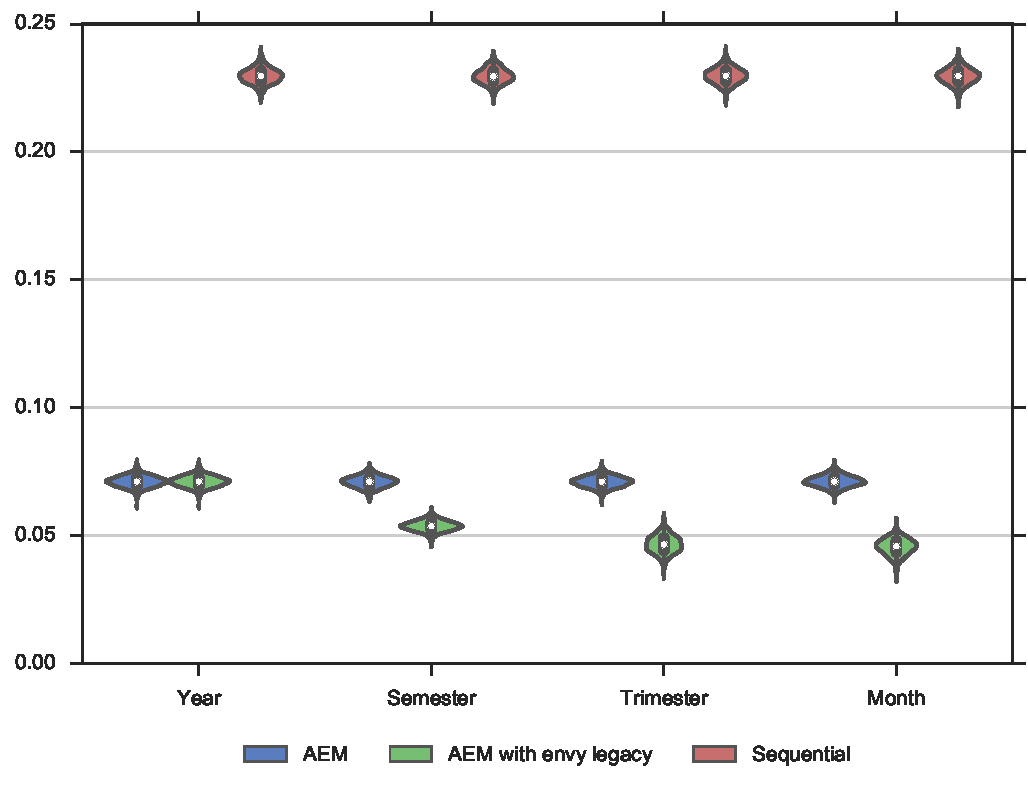
\includegraphics[width=0.5\linewidth]{../figs/quotas/single_effic_0.pdf}
	}
	\subfloat[24\% misclassification error \label{SUBFIG-quotas_effic}]{
		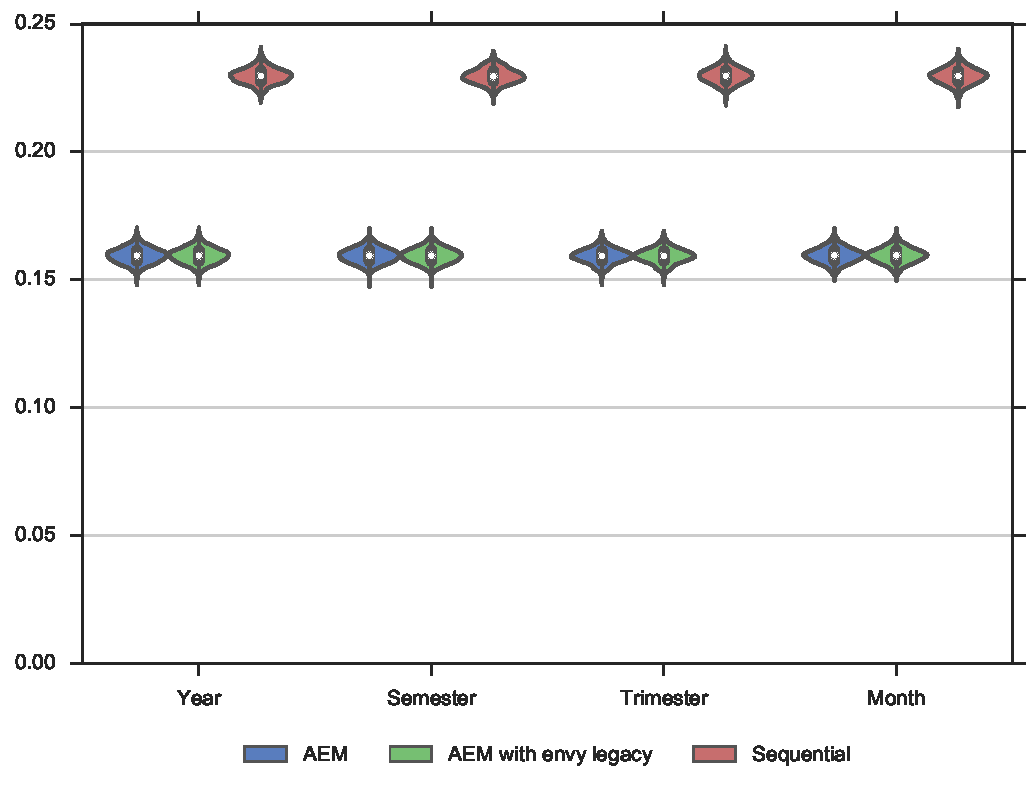
\includegraphics[width=0.5\linewidth]{../figs/quotas/single_effic_24.pdf}
	}%
	\end{center}
	{\footnotesize {\sc Notes:}---We ...}
\end{figure}

Figure \ref{FIG-quotas} shows 

- Show distribution of shares at refugee N
- outperfoms sequential
- if allow for legacy, smaller is better
- intuition: If flows of refugee random, smaller areas "in the game" for longer the smaller the quotas periods are
- results for fairness similar with or without legacy, results appear in the appendix.

\bibliographystyle{aer}
\bibliography{immigration}

\end{document}